\documentclass{beamer}
\usepackage{amsmath}
\usepackage{amsfonts}
% Calligraphic fonts
\newcommand{\calA}{{\cal A}}
\newcommand{\calB}{{\cal B}}
\newcommand{\calC}{{\cal C}}
\newcommand{\calD}{{\cal D}}
\newcommand{\calE}{{\cal E}}
\newcommand{\calF}{{\cal F}}
\newcommand{\calG}{{\cal G}}
\newcommand{\calH}{{\cal H}}
\newcommand{\calI}{{\cal I}}
\newcommand{\calJ}{{\cal J}}
\newcommand{\calK}{{\cal K}}
\newcommand{\calL}{{\cal L}}
\newcommand{\calM}{{\cal M}}
\newcommand{\calN}{{\cal N}}
\newcommand{\calO}{{\cal O}}
\newcommand{\calP}{{\cal P}}
\newcommand{\calQ}{{\cal Q}}
\newcommand{\calR}{{\cal R}}
\newcommand{\calS}{{\cal S}}
\newcommand{\calT}{{\cal T}}
\newcommand{\calU}{{\cal U}}
\newcommand{\calV}{{\cal V}}
\newcommand{\calW}{{\cal W}}
\newcommand{\calX}{{\cal X}}
\newcommand{\calY}{{\cal Y}}
\newcommand{\calZ}{{\cal Z}}

% Sets:
\newcommand{\setA}{\textsf{A}}
\newcommand{\setB}{\textsf{B}}
\newcommand{\setC}{\textsf{C}}
\newcommand{\setD}{\textsf{D}}
\newcommand{\setE}{\textsf{E}}
\newcommand{\setF}{\textsf{F}}
\newcommand{\setG}{\textsf{G}}
\newcommand{\setH}{\textsf{H}}
\newcommand{\setI}{\textsf{I}}
\newcommand{\setJ}{\textsf{J}}
\newcommand{\setK}{\textsf{K}}
\newcommand{\setL}{\textsf{L}}
\newcommand{\setM}{\textsf{M}}
\newcommand{\setN}{\textsf{N}}
\newcommand{\setO}{\textsf{O}}
\newcommand{\setP}{\textsf{P}}
\newcommand{\setQ}{\textsf{Q}}
\newcommand{\setR}{\textsf{R}}
\newcommand{\setS}{\textsf{S}}
\newcommand{\setT}{\textsf{T}}
\newcommand{\setU}{\textsf{U}}
\newcommand{\setV}{\textsf{V}}
\newcommand{\setW}{\textsf{W}}
\newcommand{\setX}{\textsf{X}}
\newcommand{\setY}{\textsf{Y}}
\newcommand{\setZ}{\textsf{Z}}

% Vectors
\newcommand{\bfa}{\mathbf{a}}
\newcommand{\bfb}{\mathbf{b}}
\newcommand{\bfc}{\mathbf{c}}
\newcommand{\bfd}{\mathbf{d}}
\newcommand{\bfe}{\mathbf{e}}
\newcommand{\bff}{\mathbf{f}}
\newcommand{\bfg}{\mathbf{g}}
\newcommand{\bfh}{\mathbf{h}}
\newcommand{\bfi}{\mathbf{i}}
\newcommand{\bfj}{\mathbf{j}}
\newcommand{\bfk}{\mathbf{k}}
\newcommand{\bfl}{\mathbf{l}}
\newcommand{\bfm}{\mathbf{m}}
\newcommand{\bfn}{\mathbf{n}}
\newcommand{\bfo}{\mathbf{o}}
\newcommand{\bfp}{\mathbf{p}}
\newcommand{\bfq}{\mathbf{q}}
\newcommand{\bfr}{\mathbf{r}}
\newcommand{\bfs}{\mathbf{s}}
\newcommand{\bft}{\mathbf{t}}
\newcommand{\bfu}{\mathbf{u}}
\newcommand{\bfv}{\mathbf{v}}
\newcommand{\bfw}{\mathbf{w}}
\newcommand{\bfx}{\mathbf{x}}
\newcommand{\bfy}{\mathbf{y}}
\newcommand{\bfz}{\mathbf{z}}


\newcommand{\bfalpha}{\boldsymbol{\alpha}}
\newcommand{\bfbeta}{\boldsymbol{\beta}}
\newcommand{\bfgamma}{\boldsymbol{\gamma}}
\newcommand{\bfdelta}{\boldsymbol{\delta}}
\newcommand{\bfepsilon}{\boldsymbol{\epsilon}}
\newcommand{\bfzeta}{\boldsymbol{\zeta}}
\newcommand{\bfeta}{\boldsymbol{\eta}}
\newcommand{\bftheta}{\boldsymbol{\theta}}
\newcommand{\bfiota}{\boldsymbol{\iota}}
\newcommand{\bfkappa}{\boldsymbol{\kappa}}
\newcommand{\bflambda}{\boldsymbol{\lambda}}
\newcommand{\bfmu}{\boldsymbol{\mu}}
\newcommand{\bfnu}{\boldsymbol{\nu}}
\newcommand{\bfomicron}{\boldsymbol{\omicron}}
\newcommand{\bfpi}{\boldsymbol{\pi}}
\newcommand{\bfrho}{\boldsymbol{\rho}}
\newcommand{\bfsigma}{\boldsymbol{\sigma}}
\newcommand{\bftau}{\boldsymbol{\tau}}
\newcommand{\bfupsilon}{\boldsymbol{\upsilon}}
\newcommand{\bfphi}{\boldsymbol{\phi}}
\newcommand{\bfchi}{\boldsymbol{\chi}}
\newcommand{\bfpsi}{\boldsymbol{\psi}}
\newcommand{\bfomega}{\boldsymbol{\omega}}
\newcommand{\bfxi}{\boldsymbol{\xi}}
\newcommand{\bfell}{\boldsymbol{\ell}}

% Matrices
\newcommand{\bfA}{\mathbf{A}}
\newcommand{\bfB}{\mathbf{B}}
\newcommand{\bfC}{\mathbf{C}}
\newcommand{\bfD}{\mathbf{D}}
\newcommand{\bfE}{\mathbf{E}}
\newcommand{\bfF}{\mathbf{F}}
\newcommand{\bfG}{\mathbf{G}}
\newcommand{\bfH}{\mathbf{H}}
\newcommand{\bfI}{\mathbf{I}}
\newcommand{\bfJ}{\mathbf{J}}
\newcommand{\bfK}{\mathbf{K}}
\newcommand{\bfL}{\mathbf{L}}
\newcommand{\bfM}{\mathbf{M}}
\newcommand{\bfN}{\mathbf{N}}
\newcommand{\bfO}{\mathbf{O}}
\newcommand{\bfP}{\mathbf{P}}
\newcommand{\bfQ}{\mathbf{Q}}
\newcommand{\bfR}{\mathbf{R}}
\newcommand{\bfS}{\mathbf{S}}
\newcommand{\bfT}{\mathbf{T}}
\newcommand{\bfU}{\mathbf{U}}
\newcommand{\bfV}{\mathbf{V}}
\newcommand{\bfW}{\mathbf{W}}
\newcommand{\bfX}{\mathbf{X}}
\newcommand{\bfY}{\mathbf{Y}}
\newcommand{\bfZ}{\mathbf{Z}}


\newcommand{\bfGamma}{\boldsymbol{\Gamma}}
\newcommand{\bfDelta}{\boldsymbol{\Delta}}
\newcommand{\bfTheta}{\boldsymbol{\Theta}}
\newcommand{\bfLambda}{\boldsymbol{\Lambda}}
\newcommand{\bfPi}{\boldsymbol{\Pi}}
\newcommand{\bfSigma}{\boldsymbol{\Sigma}}
\newcommand{\bfUpsilon}{\boldsymbol{\Upsilon}}
\newcommand{\bfPhi}{\boldsymbol{\Phi}}
\newcommand{\bfPsi}{\boldsymbol{\Psi}}
\newcommand{\bfOmega}{\boldsymbol{\Omega}}


% Blackboard Bold:
\newcommand{\bbA}{\mathbb{A}}
\newcommand{\bbB}{\mathbb{B}}
\newcommand{\bbC}{\mathbb{C}}
\newcommand{\bbD}{\mathbb{D}}
\newcommand{\bbE}{\mathbb{E}}
\newcommand{\bbF}{\mathbb{F}}
\newcommand{\bbG}{\mathbb{G}}
\newcommand{\bbH}{\mathbb{H}}
\newcommand{\bbI}{\mathbb{I}}
\newcommand{\bbJ}{\mathbb{J}}
\newcommand{\bbK}{\mathbb{K}}
\newcommand{\bbL}{\mathbb{L}}
\newcommand{\bbM}{\mathbb{M}}
\newcommand{\bbN}{\mathbb{N}}
\newcommand{\bbO}{\mathbb{O}}
\newcommand{\bbP}{\mathbb{P}}
\newcommand{\bbQ}{\mathbb{Q}}
\newcommand{\bbR}{\mathbb{R}}
\newcommand{\bbS}{\mathbb{S}}
\newcommand{\bbT}{\mathbb{T}}
\newcommand{\bbU}{\mathbb{U}}
\newcommand{\bbV}{\mathbb{V}}
\newcommand{\bbW}{\mathbb{W}}
\newcommand{\bbX}{\mathbb{X}}
\newcommand{\bbY}{\mathbb{Y}}
\newcommand{\bbZ}{\mathbb{Z}}




\setbeamertemplate{navigation symbols}{}

\title{ECE 417/598: Image formation}
\author{Vikas Dhiman}
\date{Feb 7, 2022}
\begin{document}
\begin{frame}
  \titlepage
  \end{frame}
\begin{frame}{Additional reference}
  Chapter 6, 7, 8 of  
  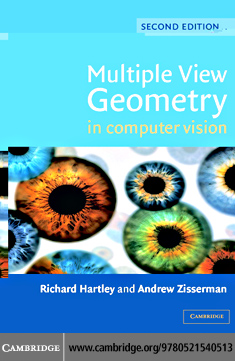
\includegraphics[width=0.3\linewidth]{media/hartley-and-zisserman.png}
  \footnote{Lookup on libgen.rs}
 \end{frame}
\begin{frame}
  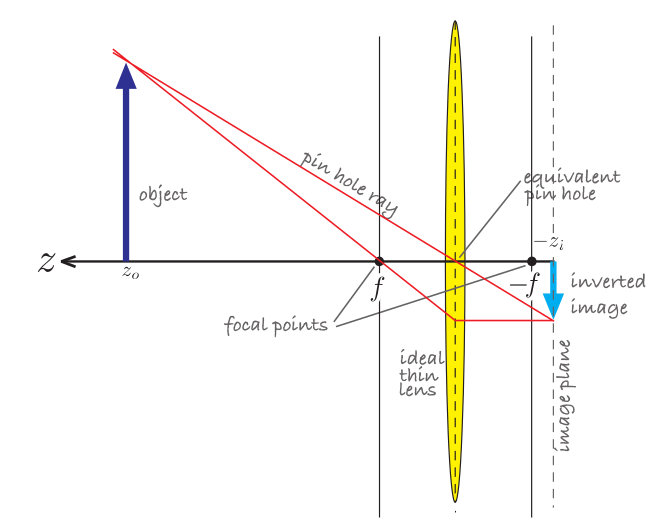
\includegraphics[width=0.48\linewidth]{media/lens-image-formation.png}
  \\
  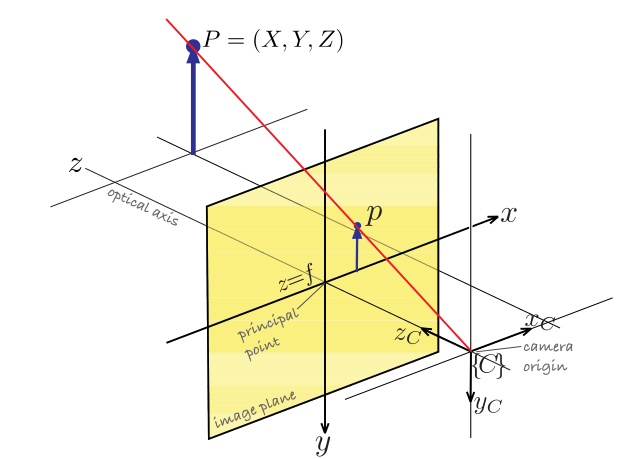
\includegraphics[width=0.48\linewidth]{media/pinhole-camera-model.png}
  \footnote{Chapter 11. Corke.}
\end{frame}
\begin{frame}
  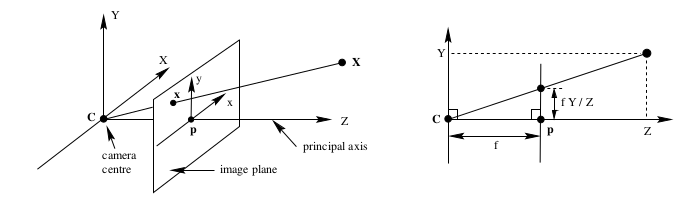
\includegraphics[width=\linewidth]{media/pinhole-camera-model-2.png}
  \footnote{Chapter 6. Hartley and Zisserman}
  \end{frame}
  \begin{frame}
    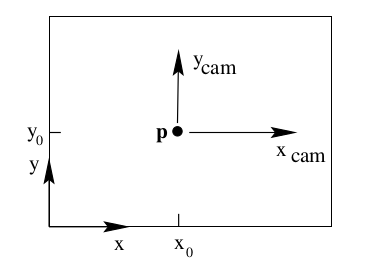
\includegraphics[width=0.4\linewidth]{media/image-center.png}
    \footnote{Chapter 6. Hartley and Zisserman}
  \end{frame}

  \begin{frame}
    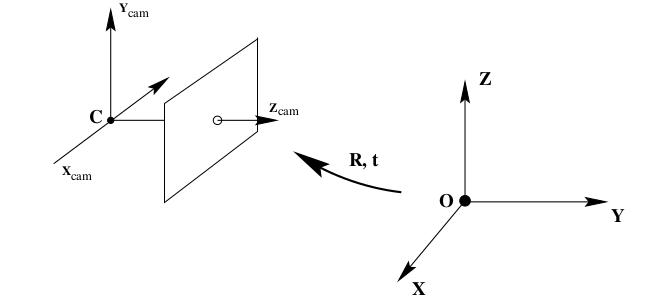
\includegraphics[width=0.4\linewidth]{media/world-camera-transformation.png}
    \footnote{Chapter 6. Hartley and Zisserman}
  \end{frame}

  \begin{frame}
    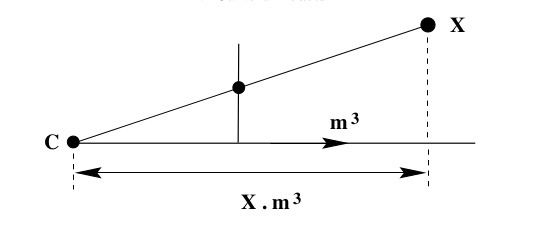
\includegraphics[width=0.4\linewidth]{media/recovering-ray-from-point.png}
    \footnote{Chapter 6. Hartley and Zisserman}
  \end{frame}

  \begin{frame}{Review}
    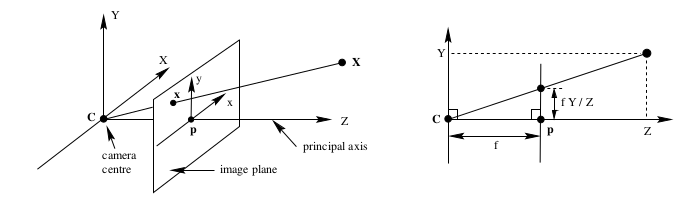
\includegraphics[width=\linewidth]{media/pinhole-camera-model-2.png}
    \newcommand{\ubfu}{\underline{\bfu}}
    \newcommand{\ubfX}{\underline{\bfX}}
    \begin{align}
      \bfK &= \begin{bmatrix}
        f_x & s & u_0 \\
        0 & f_y & v_0 \\
        0 & 0 & 1 \\
      \end{bmatrix}
      \\
      \bfu &= [x, y]^\top \\
      \ubfX &= [X, Y, Z]^\top\\
      \ubfu &= [\bfu^\top, 1]^\top \\
      \ubfu &= K \ubfX
      \end{align}
    \end{frame}

  \begin{frame}{A numerical example}
    Image is a grid of numbers. The vale in the grid represents intensity values.
    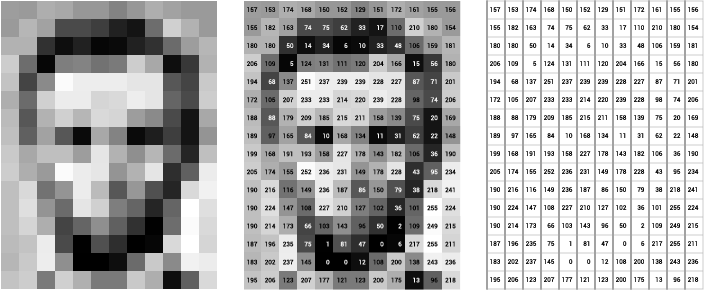
\includegraphics[width=\linewidth]{media/image-as-a-matrix.png}
  \end{frame}

  \begin{frame}
    A Depth Image is an array of numbers. The value in the grid represents
    intensity values.\\
    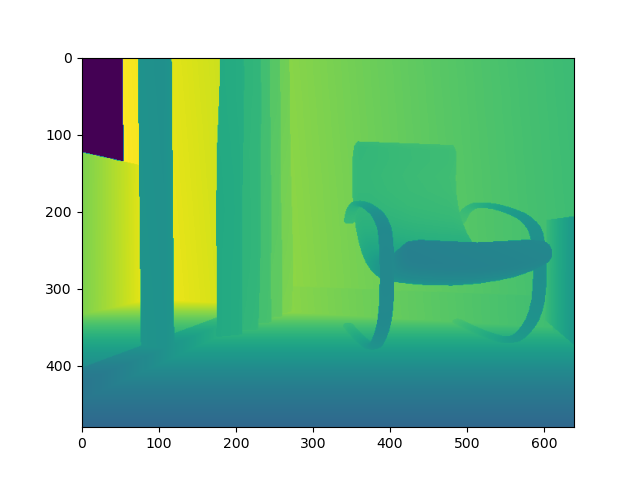
\includegraphics[width=0.45\linewidth]{media/00000-depth.png}%
    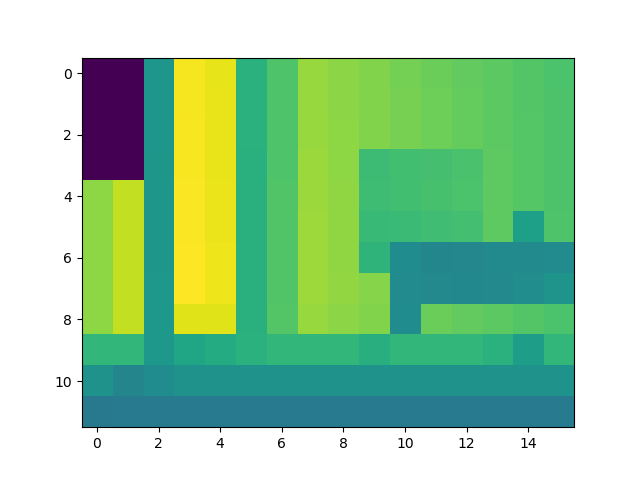
\includegraphics[width=0.45\linewidth]{media/00000-depth-lowres.png}
  \end{frame}

  
  \begin{frame}
    From what we have learned, how can we convert the depth image to a point cloud?
    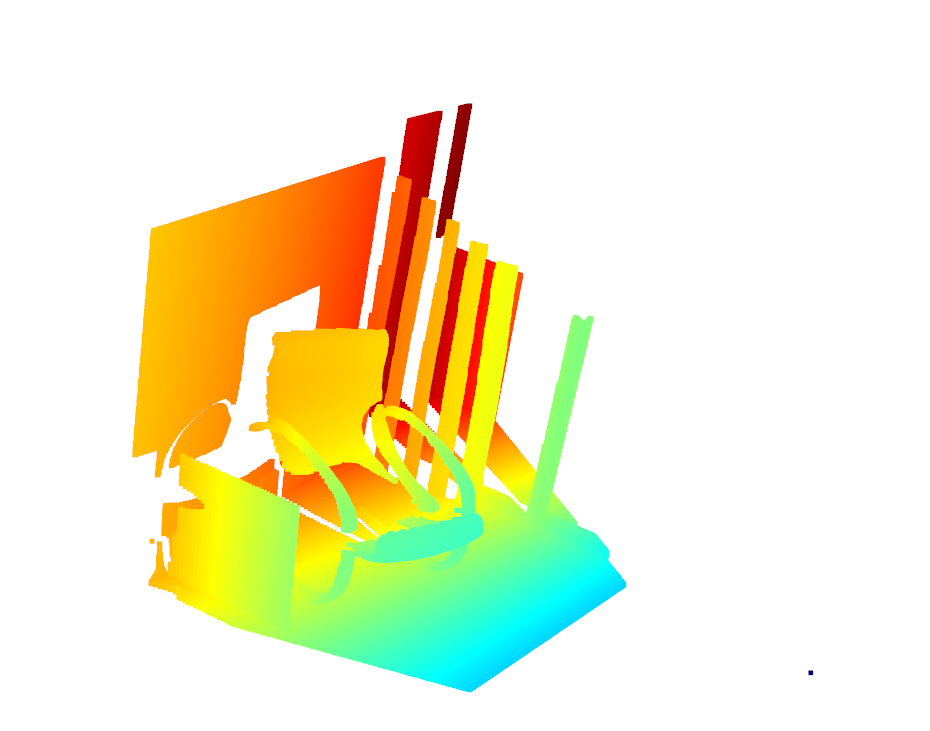
\includegraphics[width=0.45\linewidth]{media/depth-image-to-point-cloud-1.png}%
    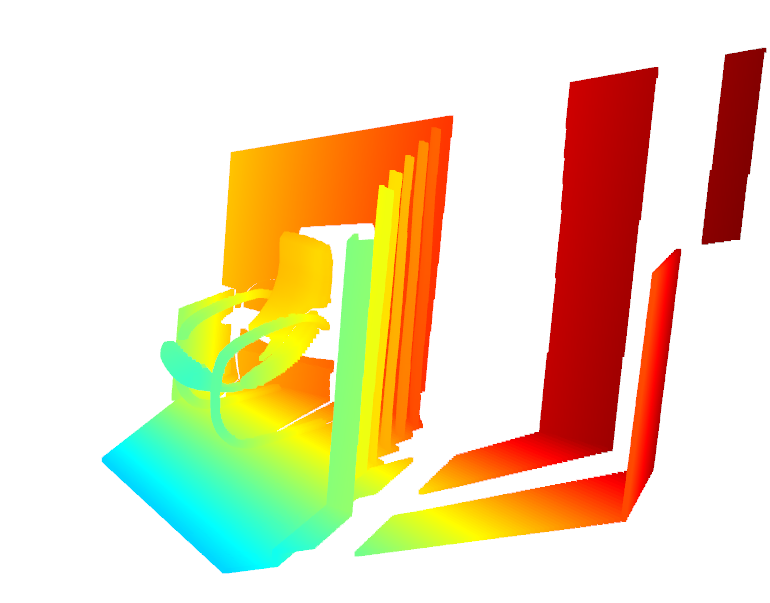
\includegraphics[width=0.45\linewidth]{media/depth-image-to-point-cloud-2.png}
  \end{frame}


  \begin{frame}{Pseudo-Inverse}
    \begin{align}
      \bfA \bfA^\dagger \bfA &=  \bfA \\
      \text{If SVD of $\bfA$ is given by } \bfA &= \bfU \Sigma \bfV^\top 
      \text{ then } \bfA^\dagger = \bfU \Sigma^{-1} \bfV^\top \\
      \text{if } \bfA \text{ is tall, then } \bfA^\dagger &= (\bfA^\top \bfA)^{-1} \bfA^\top \\
      \text{if } \bfA \text{ is fat, then } \bfA^\dagger &=  \bfA^\top (\bfA \bfA^\top)^{-1}
    \end{align}
  \end{frame}

  \begin{frame}{Points as rays: aka Prospective geometry}
  \end{frame}

  \begin{frame}
    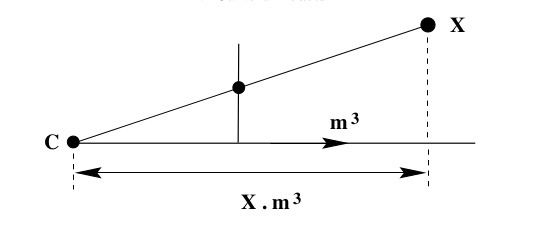
\includegraphics[width=0.4\linewidth]{media/recovering-ray-from-point.png}
    \footnote{Chapter 6. Hartley and Zisserman}
  \end{frame}

  \begin{frame}{Vanishing Point}
    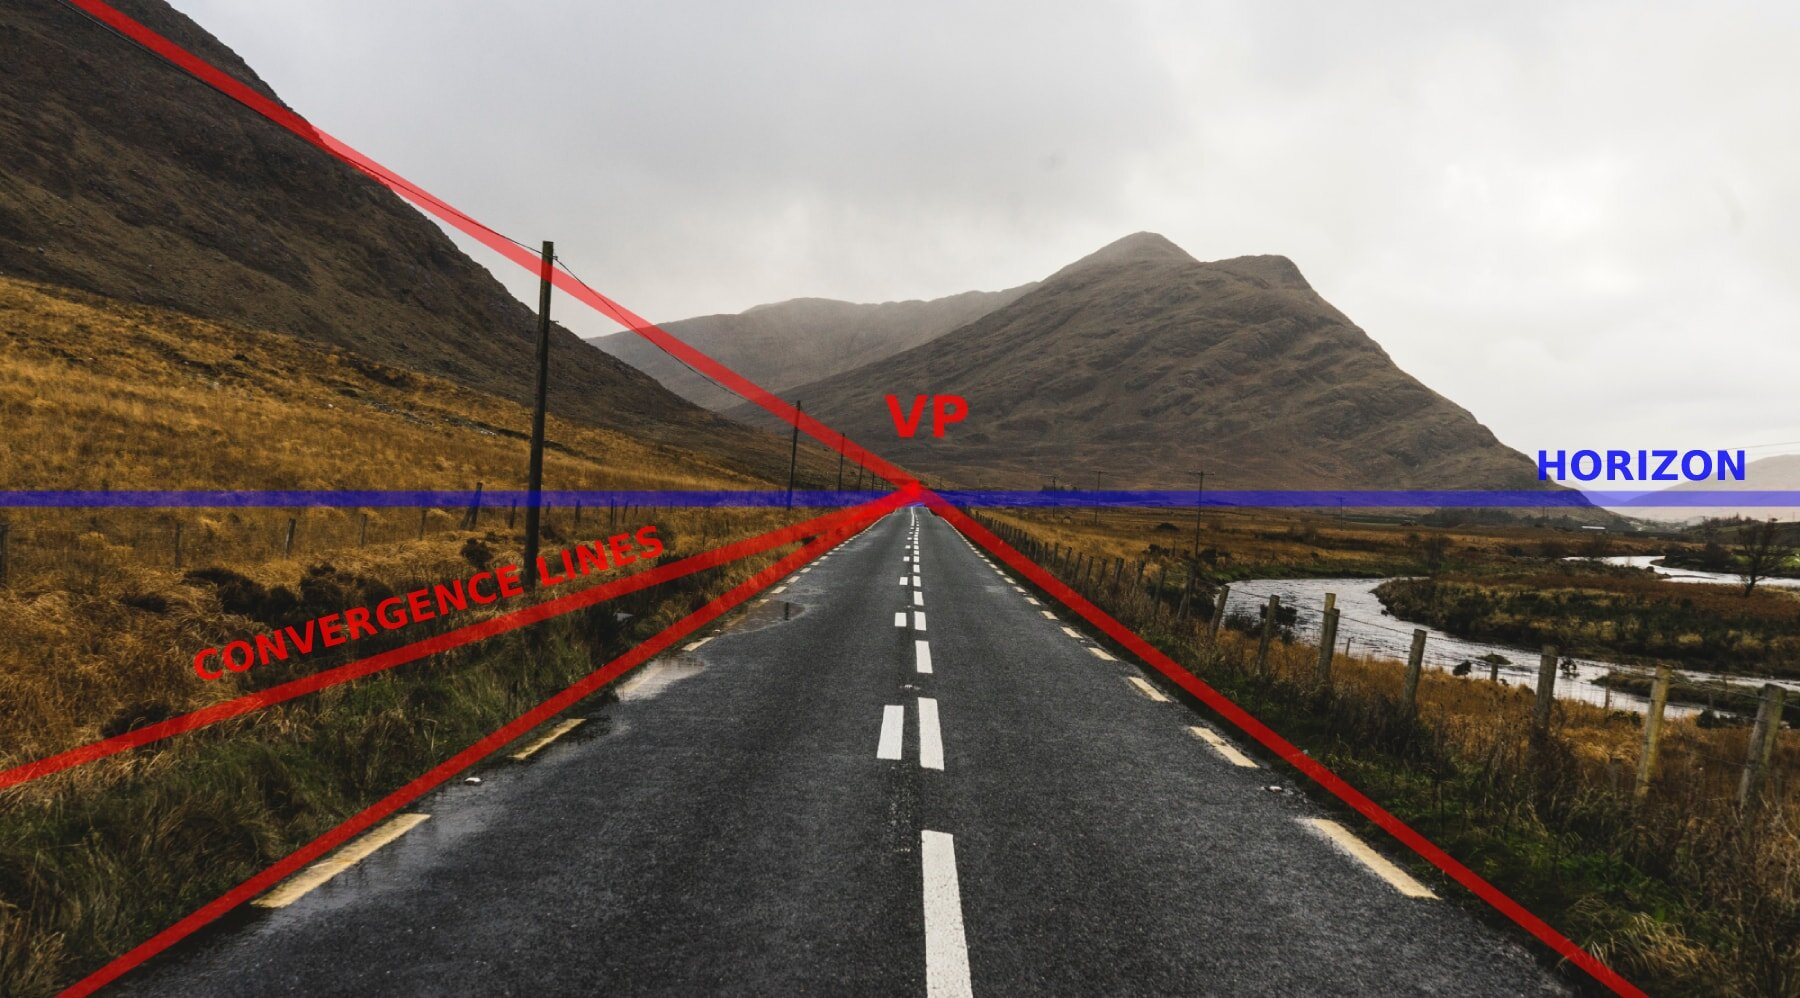
\includegraphics[width=0.7\linewidth]{media/vanishing-lines.jpeg}
    \\
    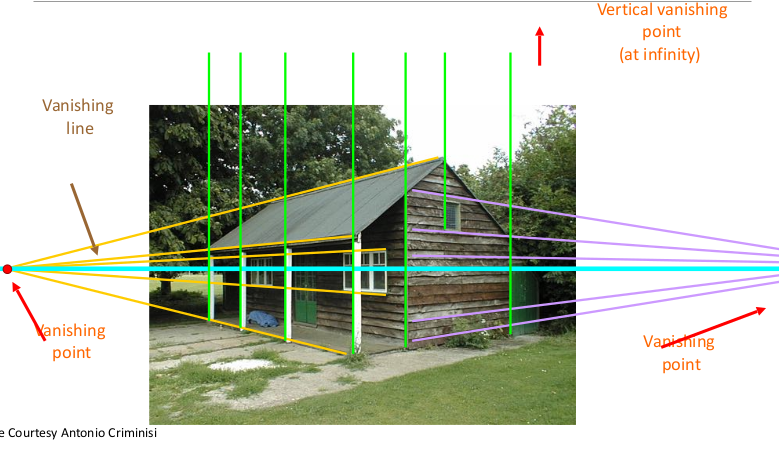
\includegraphics[width=0.7\linewidth]{media/vanishing-points.png}
  \end{frame}

  \begin{frame}{Vanishing Point}
    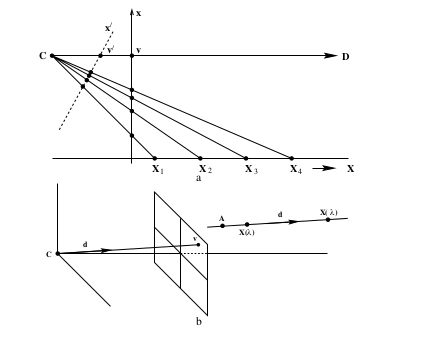
\includegraphics[width=0.5\linewidth]{media/vanishing-point-formation.png}
  \end{frame}

\end{document}